\chapter{Marco Teórico}

 En este capitulo se aborda el marco teórico necesario para comprender más fácilmente el desarrollo de los capítulos posteriores. Se analiza el problema del tráfico en general, los simuladores y la teoría detrás del algoritmo a utilizar.

\section{Problema del tránsito vehicular}

En gran parte del mundo se está produciendo un crecimiento sostenido del parque automotor lo que ocasiona una serie de problemas que afectan la calidad de vida de las personas relacionados con el agravamiento de las congestiones vehiculares \citep{Cepal2003}.

Este problema tiene un gran impacto en el desarrollo de las ciudades por lo que es un componente principal en los planes estratégicos para su crecimiento.

La congestión ocasiona una progresiva merma en la velocidad promedio de circulación, lo que incrementa la duración de los viajes, aumenta el consumo de combustible y la contaminación atmosférica y sonora, lo que repercute directamente en la salud de las personas. 
además se genera una exigencia en las vías de tránsito que ocasiona un deterioro mayor de calles y rutas.

Uruguay no escapa a este fenómeno en particular Montevideo, donde el aumento del parque automotor está en ascenso constante desde el 2005 \citep{INE2014} 
Y según proyecciones el crecimiento seguiría en un promedio de 4.5\% anual hasta el 2020. \citep{BBVA2013}

Esto viene de la mano con el sostenido aumento de las ventas de vehículos  desde el 2003 \citep{Autoanuario2014}

Los expertos indican que la congestión ya está instalada y la infraestructura vial no acompasó este crecimiento. además se indica que Montevideo es la ciudad con más semáforos por automóvil en Latinoamerica. Con más de 620 cruces semaforizados, alguno de los cuales no están coordinados.\citep{Subrayado2013}

Por todo esto es relevante el tema de la sincronización de semáforos para agilizar el tránsito y no generar congestiones, aumentando la velocidad promedio de los viajes y mejorando las perspectivas de desarrollo de la ciudad así como la calidad de vida de sus habitantes.

\section{Corredor Garzón}
El corredor Garzón se ubica en Montevideo Uruguay, fue construido como parte de un plan de movilidad que incluye otros 4 corredores. 
Presenta un carril exclusivo para ómnibus y preferenciales
http://www.montevideo.gub.uy/ciudadania/stm-transporte-metropolitano/plan-de-movilidad/corredores

Tiene 6km de largo , extendiéndose desde ...  hasta ..
%http://www.montevideo.gub.uy/sites/default/files/articulo/corredor_garzon.pdf

Agregar mapa y poner referencia de donde se saco

Los problemas de sincronización de semáforos fueron admitidos en varias publicaciones.

18 diciembre 2013 - Corredor Garzón lucha contra el tiempo %http://www.elpais.com.uy/informacion/imm-corredor-garzon-tiempos-cambios.html
Dice que antes de Garzon se demoraba promedio 18 minutos, y al inaugurar el corredor 30 minutos. Después se mejoro algo para equilibrar los tiempos
Para el jerarca, eso se dio "con la diferencia de que hoy hay 15 semáforos más y se ganó en seguridad". En concreto, tras la obra, se pasó de tener 5 semáforos a 20. Según Campal, su des-coordinación inicial, entre otros aspectos, fue lo que provocó tales demoras, generando malestar en los usuarios.
inversión de 60 millones


4 agosto 2013 - Garzon desde un omnibus %http://www.elpais.com.uy/informacion/corredor-garzon-visto-bus.html


30 julio 2013  - Intendetnta admite errores %http://www.elpais.com.uy/informacion/garzon-olivera-admitio-errores.html
La intendenta admte errores y dice: no se ha logrado sincronizar los semáforos. Hay un tema con el software,(y) la empresa subcontratada no ha dado los resultados esperados


Abril 2013 - Otro Corredor con obras paralizadas por criticas a GArzon
%http://www.elpais.com.uy/informacion/marcha-atras-en-corredor-agraciada.html




\section{Algoritmos Evolutivos}

Uno de los puntos importantes del presente trabajo son los algoritmos genéticos por lo que se dedica esta sección para  brindar un repaso por los conceptos y definiciones necesarias para comprender el desarrollo posterior de la solución.

Los algoritmos evolutivos son métodos no determinísticos que se inspiran en la evolución natural de las especies utilizando conceptos como población, cruzamiento, mutación, selección, etc. Estos se utilizan para resolver problemas de optimización y búsqueda, entre otros \citep{Nesmachnow2002}.

Es una técnica iterativa que busca en cada paso mejorar las soluciones por medio de operadores basado en un criterio predefinido para maximizar o minimizar.

Este tipo de solución ha demostrado su utilidad en una amplia variedad de problemas complejos.


\subsection{Algoritmos Genéticos}
El algoritmo genético es uno de los más populares dentro de los algoritmos evolutivos.

La idea base es que partiendo de una población inicial de individuos se seleccionan los mejores en base a su aptitud respecto a solucionar el problema y estos se utilizan para generar nuevos individuos ya sea por combinación o modificación. Por tanto en cada paso obtenemos mejores soluciones hasta detenernos usando un criterio de parada ya sea el número de iteraciones o cuando ya no se puede mejorar más la solución.

Un individuo es una codificación de la solución que resuelve el problema.
La población inicial puede generarse aleatoriamente o basándose en algún conocimiento previo.
La función de evaluación indica que tan buena o apta es una solución en comparación con las demás.
En cada iteración la cual se llama generación se aplican operadores de cruzamiento estos son formas de combinar a los individuos para obtener otros que potencialmente sean una mejor solución y también cambios aleatorios sobre los individuos llamado mutación.

Por tanto se van seleccionando, combinando y cambiando las mejores soluciones en un proceso que va obteniendo mejores soluciones.
El criterio de parada nos indica cuando termina este proceso, ya sea por que se alcanzó un número de generaciones predefinidos o por que la mejora no es evidente. Al final se devuelve la mejor solución encontrada en todo el proceso.

Hay que indicar que no es una técnica exacta pero si logra muy buenas aproximaciones y es muy buena en problemas complejos por su flexibilidad y robustez. 


\subsubsection{Representación de soluciones}
No podemos trabajar directamente sobre las soluciones, por lo que tenemos que codificarlas en un modelo que nos sirva para poder aplicar el algoritmo.
La inspiración biológica se ve en los nombres que adopta esta representación, llamada Cromosoma que es un vector de genes y cada valor de un gen se llama alelo.
En general se codifica un vector de números binarios o reales de largo fijo, lo que facilita la aplicación de los operadores.

\subsubsection{Función de Evaluación} 
Indica que tan bueno es un individuo para resolver el problema en cuestión con un valor conocido como Fitness. Este se utiliza para seleccionar a los mejores y de esta forma guiar la exploración hacia la mejor solución.
Se deben tener en cuenta las restricciones del problema para que las soluciones no factibles no sobrevivan.
En general es donde se consume el mayor tiempo del algoritmo en comparación con los demás operadores.

\subsubsection{Operador de Selección}
Existen diversos operadores de selección , su función es que las mejores características de los individuos se mantengan en las siguientes generaciones.
Los tipos más populares son:

\begin{itemize}
	\item Ruleta: También conocida como selección proporcional elige aleatoriamente individuos en la cual la probabilidad de selección es proporcional al valor de fitness.
	\item Torneo: Se elige aleatoriamente un determinado número de individuos los cuales compiten entre si.
	\item Elitismo: Los mejores individuos son mantenidos entre las generaciones.
\end{itemize}

\subsubsection{Cruzamiento}
Su función es combinar individuos para lograr mejores soluciones. 
Existe una tasa que se puede modificar para indicar la probabilidad de que se realice el cruzamiento.

\begin{itemize}
	\item Cruzamiento de un punto: A partir de dos padres se selecciona un punto al azar de los cromosomas obteniendo dos trozos que se combinan para obtener dos hijos. Se explica en la figura ~\ref{fig:cruzamiento1}
	\item Cruzamiento multipunto: El método anterior se puede generalizar para obtener más puntos de corte y más recombinaciones.
\end{itemize}

\begin{figure}[h]
	\centering
	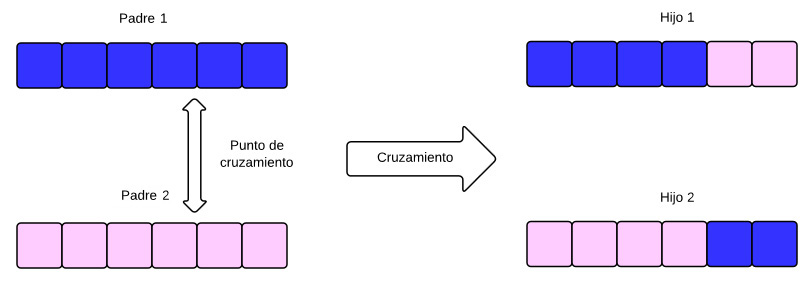
\includegraphics[width=\textwidth]{Figures/cruzamiento1}
	\caption{Cruzamiento de un punto}
	\label{fig:cruzamiento1}
\end{figure}

\subsubsection{Mutación} 
Indica el método utilizado para modificar un individuo, esto se realiza para lograr más diversidad y no caer en máximos locales. En general aplica una modificación aleatoria en el cromosoma.También hay una tasa de probabilidad, en general es baja. En el caso de un cromosoma binario se aplica la inversión sobre un alelo.

\begin{figure}[h]
	\centering
	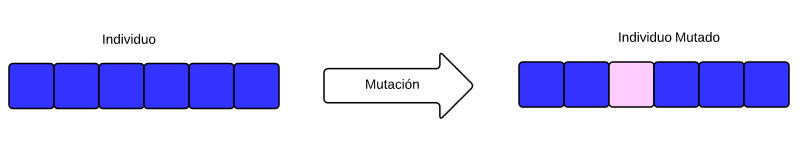
\includegraphics[width=1\linewidth]{Figures/mutacion1}
	\caption{Mutacion por inversión binaria}
	\label{fig:mutacion1}
\end{figure}


\subsubsection{Reemplazo} 
Se indica cual es el criterio que debemos tomar para generar una nueva población, ya sea tomando solo los hijos creados o comparando también con los padres o aplicando algún otro criterio.

\subsubsection{Criterio de parada} 
Indica cuando debe terminar el algoritmo, puede ser definiendo un número fijo de generaciones o analizando si el mejor valor de fitness se mantiene relativamente constante durante un número determinado de generaciones.

\subsection{Funcionamiento}

El esquema básico de funcionamiento es el siguiente:


\begin{algorithm}%[!ht]
	\caption{Algoritmo Genético}
	\label{alg:algoritmo_genetico_simple}
	\begin{algorithmic} [1] 
		{
			%\small
			\STATE {Inicializo( Pob(0))}
			\STATE \texttt{generacion} = 0
			\WHILE {\text{No llegue al criterio de parada}}
			\STATE {Evaluar Pob(generacion)}
			\STATE {Padres = Seleccionar(Pob(generacion))}
			\STATE {Hijos = Cruzamiento(Padres) y Mutacion(Padres)}
			\STATE {NuevaPob = Reemplazar Pob(generacion) con Hijos}
			\STATE \texttt{generacion}++
			\ENDWHILE
			\RETURN Mejor solución
		}
	\end{algorithmic}
\end{algorithm}



% ctrl+t comenta
%\begin{algorithm}%[!ht]
%	\caption{Genetic Algorithm}
%
%	\begin{algorithmic} [1] 
%		{
%
%			\STATE {Init( Pop(0))}
%			\STATE \texttt{generation} = 0
%			\WHILE {\text{NOT Stop Criteria}}
%			\STATE {Evaluate Pop(generation)}
%			\STATE {Parents = Selection(Pop(generation))}
%			\STATE {Children = Crossover(Parents) and Mutation(Parents)}
%			\STATE {NewPop = Replace Pop(generation) with Children}
%			\STATE \texttt{generation}++
%			\ENDWHILE
%			\RETURN Best solution
%		}
%	\end{algorithmic}
%\end{algorithm}


\subsection{Algoritmos genético multiobjetivo}

En este caso se busca una solución que satisfaga de forma simultánea tanto las restricciones del problema como varios objetivos distintos.



\subsection{Algoritmo Genético Paralelo}
Los problemas complejos suelen requerir una alta demanda computacional por lo que aplicar técnicas de paralelización es útil para lograr tiempos de ejecución menores.

Existen varios niveles de paralelización ya sea a nivel global enfocándonos en paralizar la función fitness, a nivel de la población, o a nivel del individuo. \citep{Nesmachnow2002}

En el caso de los algoritmos genéticos gran parte del tiempo se ocupa en la etapa de evaluación, por esta razón es un buen método para distribuir la carga en varios procesadores para que las evaluaciones se realicen en paralelo.


\subsection{Maestro-Esclavo}

En este modelo un proceso maestro es el encargado de realizar los operadores básicos del algoritmo y distribuir a procesos esclavos la evaluación de la función fitness para un conjunto de individuos, el esclavo devuelven el resultado y luego el maestro es el encargado de continuar ejecutando los operadores.

De este modo aumenta la eficiencia computacional del algoritmo ya que una de las funciones más costosas es distribuida entre varios nodos.

\begin{figure}[H]
	\centering
	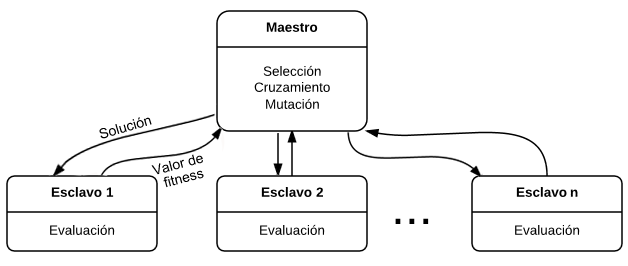
\includegraphics[width=0.7\linewidth]{Figures/diagrama-master-slave}
	\caption[Modelo Maestro-Esclavo]{Modelo Maestro-Esclavo}
	\label{fig:diagrama-master-slave}
\end{figure}



\section{Simulación}

\subsection{Simuladores de tráfico}
Los simuladores de tráfico son programas que simulan el movimiento de vehículos sobre una red de calles, es una herramienta muy usada en la investigación de tráfico vehicular; así como estudio de congestiones o análisis de impacto que tendrán nuevas infraestructuras.  Las razones para usar una simulación son varias, entre ellas se encuentra  la rapidez, ya que la simulación se puede realizar en tiempo mucho más rápidos que en la realidad, el costo en dinero pues no estamos afectando el escenario real  y tampoco tenemos que modificar o detener el escenario real para probar nuevos parámetros. además nos sirve para poder prever situaciones que podrían darse bajo determinadas circunstancias.

Los simuladores se pueden dividir en microscópicos o macroscópicos según el nivel de detalle de la simulación. Un simulador macroscópico modela  el tráfico vehicular como un fluido. En cambio un simulador microscópico simula el movimiento de cada vehículo según sus características particulares.

SUMO\citep{SUMO} es uno de los simuladores abiertos más populares, es microscópico y utiliza una serie de archivos  XML que representan las rutas, los vehículos y el tráfico.  

Cuanto más crece el número de vehículos y la complejidad de la red de mapas más difícil se hace crear la entrada básica que necesita el simulador. Aunque existen diversas herramientas que ayudan a este proceso aún se requiere un trabajo manual para el acondicionado de estos archivos.

En las siguientes secciones se muestra más en detalle algunas de sus funcionalidades y características.


\subsection{Modelo de tráfico }
Esta es la representación de la circulación de vehículos, aquí exponemos algunos de los más populares. 

Aleatorios: Genera diferentes recorridos que seguirán los vehículos aleatoriamente

JTR (junction turning ratio) : basados en probabilidades en los cruces  es decir cuando un vehículo llega a un cruce tiene cierta probabilidad de seguir o doblar.
 
Basado en áreas:  Se especifican áreas como un conjunto de calles y se realizan recorridos entre ellas.


Basado en Actividad: Se especifica la cantidad de casas, vehículos y población en un determinado lugar y el modelo genera la densidad de tráfico que se producirá basado en los tipos de actividades que se realizan comúnmente como ir al trabajo, hacer las compras, ir a la escuela,  etc

Definido por el usuario: que permiten determinar la ruta de los vehículos con mayor detalle.

\subsection{Representaciones}

\subsubsection{Red de calles}
La red de calles se representa como un grafo dirigido en un archivo xml con extensión .net.xml . Allí se especifican los nodos, y vértices así como sus atributos. También se representan los semáforos. Esto  se genera utilizando una herramienta  para convertir un mapa al formato que SUMO utiliza.

\subsubsection{Representación tráfico}
En este caso también se utiliza un archivo xml donde se definen las rutas y los recorridos. Un recorrido representa el movimiento de un vehículo de un punto inicial hacia un punto final (El recorrido se hacen en tiempo de ejecución utilizando el camino más corto basado en el tráfico). 


\subsubsection{Representación del tiempo}
El tiempo se representa como una serie de pasos discretos, cada uno durando un segundo. Este valor se puede modificar aunque es recomendado dejarlo así para que sea consistente.


\subsubsection{Tipos de vehículos}
Se pueden crear diferentes tipos de vehículos especificando propiedades como largo, velocidad máxima,  aceleración, color, etc. También cuenta con vehículos por defecto como buses, camiones o automóviles.

\subsection{Configuración de la simulación}

En esta sección se realiza un resumen sobre los pasos realizados para tener los elementos necesarios para realizar la simulación.

\subsubsection{Diseño del mapa}


El mapa base de la zona proviene de Open Street Map \citep{OSM}, luego se cotejó su exactitud con Google Maps y Bing Maps.

\begin{figure}[H]
\centering
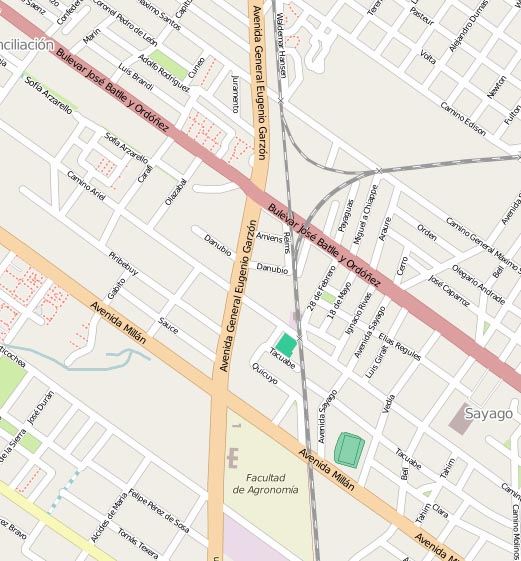
\includegraphics[width=0.7\linewidth]{Figures/osm_garzon}
\caption{Tramo del mapa de Garzon de OSM}
\label{fig:osm_garzon}
\end{figure}


Se utilizó la herramienta netconvert para convertirlo al formato que SUMO acepta. 
Para esto se realizaron varios ajustes editando los archivos xml para corregir errores en las calles, cruces y conexiones para que fuese fiel a la realidad y mantuviera la compatibilidad con SUMO.


\begin{figure}[H]
\centering
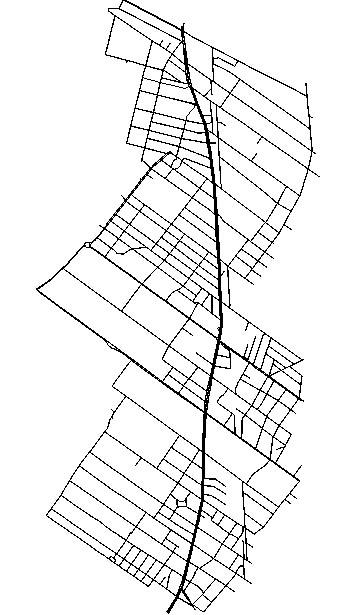
\includegraphics[width=0.5\linewidth]{Figures/mapa_sumo}
\caption{Mapa cargado en SUMO luego del modelado y procesamiento}
\label{fig:mapa_sumo}
\end{figure}



\subsubsection{Trabajo de campo realizado}
Al no contar con datos públicos sobre la configuración de los semáforos de la zona, realizamos un revelamiento in-situ con las siguientes características.

Se seleccionaron 5 cruces que presentan diferentes características para poder modelar las variantes tanto de cruces con alto tráfico, medio y bajo. 
Estos son: Camino Ariel, Battle y Ordoñez, Plaza Videla, Camino Colman y Aparicio Saravia.

Se eligió el día miércoles, que estuviera soleado y entre las 15 y 17 horas para no tener los sesgos que se producen los fines de semana o días de lluvia.
Se realizaron filmaciones de 30 min en los cruces y luego se analizaron los vídeos para realizar el conteo manual con la posibilidad de enlentecer el vídeo para mayor facilidad. Luego se completa una planilla excel donde se tiene la información de vehículos que recorren Garzón, la calle que cruza y los que doblan. También discriminamos entre vehículos y ómnibus que recorren Garzón.

\begin{figure}[H]
\centering
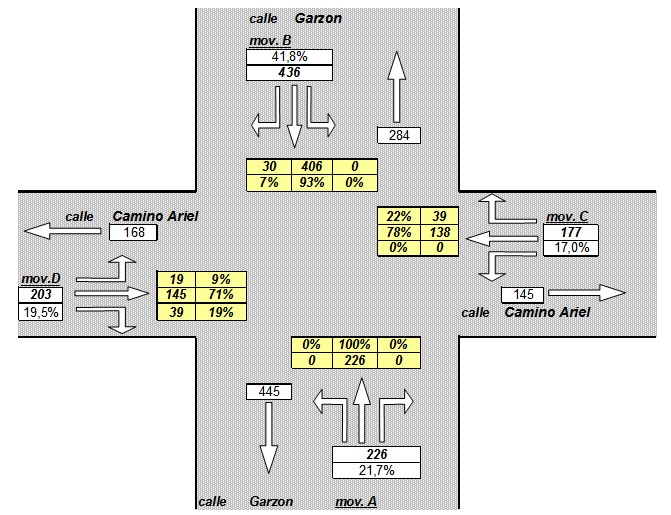
\includegraphics[width=0.7\linewidth]{Figures/conteo_hoja}
\caption{Planilla electrónica para el conteo manual en Camino Ariel}
\label{fig:conteo_hoja}
\end{figure}


además se realizaron recorridas de punta a punta del corredor a una velocidad constante para verificar los tiempos obtenidos en la simulación para este recorrido.

Para obtener la configuración de los semáforos se realizo un recorrido en bicicleta por el corredor cronometrando la duración del tiempo en cada esquina de cada semáforo. Tanto de ida como de vuelta para corroborar que fueran correctos. Estos tiempos fueron verificados por los vídeos obtenidos.


\newpage
\subsubsection{Creación del modelo del tráfico}

Con los datos relevados se creo un modelo vehicular de la ciudad [poner el mapa] que brinda una aproximación sobre la densidad de tráfico y la velocidad promedio de circulación.

Se utilizó el programa Traffic Modeler \citep{TrafficModeler} con lo que se logra generar modelos de tráfico complejo de manera visual y sencilla. Se optó por un modelo de movilidad entre áreas lo que permite una buena granularidad al especificar la densidad de tráfico.


\begin{figure}[H]
\centering
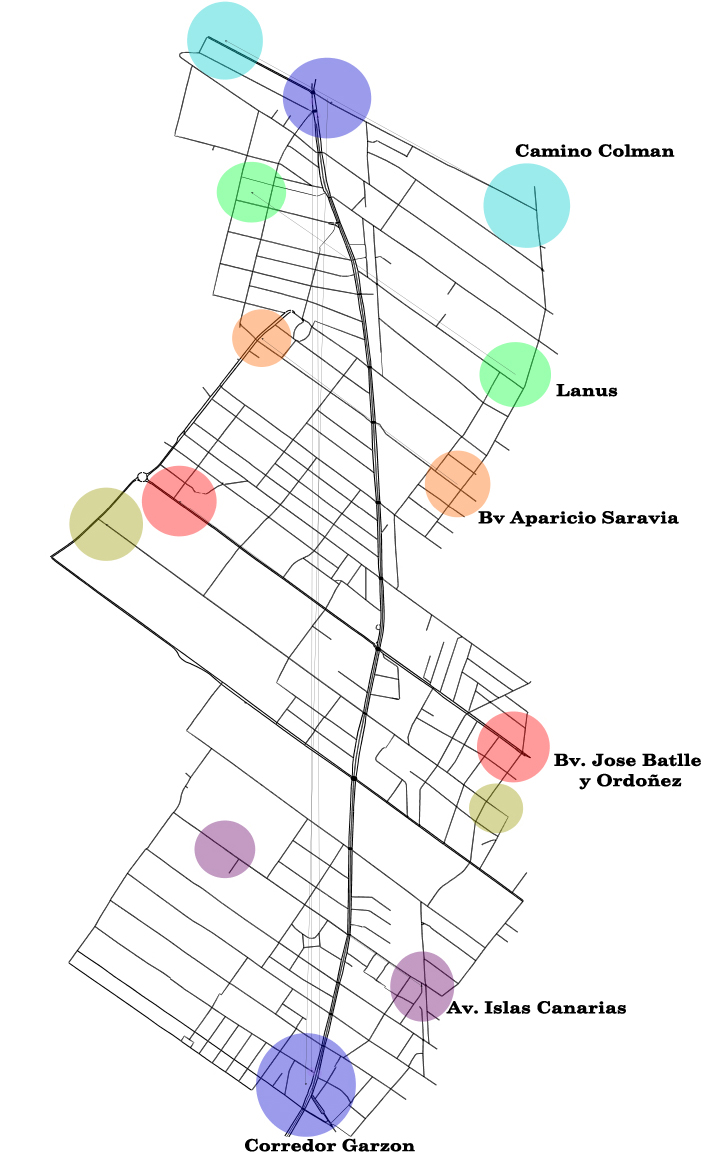
\includegraphics[width=0.4\linewidth]{Figures/areaflow1}
\caption{Mapa del TrafficModeler con las áreas de tráfico. Círculos del mismo color indican tráfico especificado entre esas áreas}
\label{fig:areaflow1}
\end{figure}


Actualmente no se cuenta con información publica relativa a la configuración de los semáforos en la ciudad, aunque cabe destacar que en el futuro se prevé crear un sistema centralizado de sincronización de semáforos. \citep{OBS01} 
En este caso se agregó la información sobre la configuración de los semáforos de los datos relevados.

Se manejaron dos tipos de vehículos autos y ómnibus cada uno con características distintas tanto de tamaño, aceleración y velocidad máxima.

Se agregaron las frecuencias y los distintos recorridos de los ómnibus obtenidos de datos públicos de la Intendencia de Montevideo \citep{IMM}
Estos incluyen las lineas urbanas  'G',  la  '409' , '522'  y  '148' . Las líneas de ómnibus suburbanas realizan  un mismo  trayecto y las generalizamos con el nombre 'A'.  
Todas  las  líneas  de  ómnibus
fueron cargadas con las paradas correspondientes y se
hicieron  variantes  en  los  viajes  dentro  de  una  misma
línea para simular el hecho de que no siempre se para en las mismas paradas.




\begin{figure}[h]
	\centering
	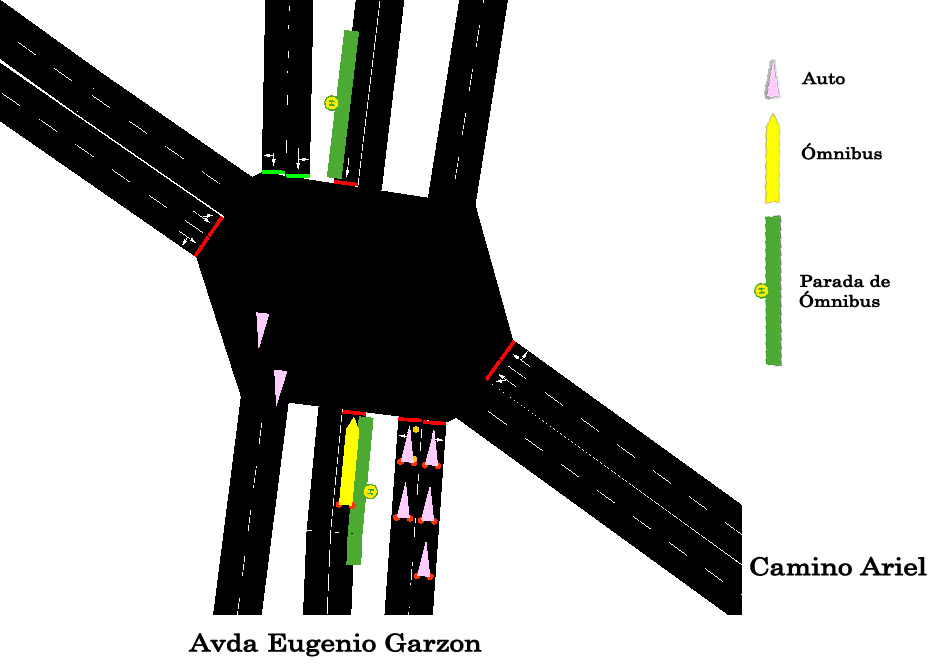
\includegraphics[width=0.7\linewidth]{Figures/sim1}
	\caption{Simulacion de tráfico en SUMO en el cruce entre Bulevar Battle y Ordoñez y el Corredor Garzon.}
	\label{fig:sim1}
\end{figure}








